\documentclass[a4paper]{article}

\usepackage[portuguese]{babel}
\usepackage[utf8]{inputenc}
\usepackage{graphicx,hyperref}
\usepackage{float}
\usepackage{listings}
\usepackage{proof,tikz}
\usepackage{algorithm2e}
\usepackage{amssymb,amsthm,stmaryrd}


\usepackage[edges]{forest}
\usetikzlibrary{automata, positioning, arrows}


\newtheorem{Lemma}{Lema}
\newtheorem{Theorem}{Teorema}
\theoremstyle{definition}
\newtheorem{Example}{Exemplo}
\newtheorem{Definition}{Definição}
\newtheorem{Fact}{Fato}


\usepackage{fancyhdr}
  \pagestyle{fancy}
  \fancyhf{}
  \lhead{Teoria da Computação}
  \rhead{Aula 23}
  \lfoot{Prof. Rodrigo Ribeiro}
  \rfoot{\thepage}
  \renewcommand{\footrulewidth}{0.4pt}
  \pagestyle{fancy}

\tikzset{
        ->,  % makes the edges directed
        >=stealth', % makes the arrow heads bold
        node distance=3cm,
        every state/.style={thick, fill=gray!10},
        initial text=$\,$
        }
  

\begin{document}

\title{Aula 23 - Indecidibilidade do problema da parada}
  \author{Rodrigo Ribeiro}

  \maketitle

  \pagestyle{fancy}


  \section*{Objetivos}

  \begin{itemize}
     \item Apresentar a demonstração de que o problema da
           parada para MTs é indecidível.
     \item Apresentar a demonstração de que o problema da
           para linguagens de programação convencionais
           é indecidível.
  \end{itemize}


  \section{O problema da parada para MTs}

  \begin{Definition}[Problema da parada para MTs]
    Dadas uma MT arbitrária $M$ e uma palavra $w$, determinar se a computação
    de $M$ para com entrada $w$.
  \end{Definition}

  Vamos mostrar que o problema da parada é indecidível, isto é, não existe
  algoritmo capaz de dar a resposta correta (lembre-se: loop não é resposta!)
  para todas as possíveis instâncias deste problema.

  \begin{Theorem}
    O problema da parada para MTs é indecidível.
  \end{Theorem}
  \begin{proof}
    Na demonstração, consideraremos que a palavra de entrada $w$ é representada
    por ela própria, isto é, $R\langle w \rangle = w$. A prova será por
    contradição.
    Suponha que exista uma MT $P$ que decida o problema da parada. Essa MT é
    apresentada na figura seguinte.
    \begin{figure}[H]
      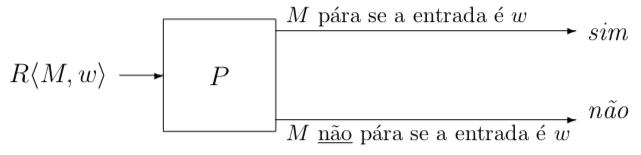
\includegraphics[scale=.4]{MTP.png}
      \centering
    \end{figure}
    A partir de $P$, pode-se construir uma MT $P'$ de forma que $P'$ entra em
    loop exatamente nas situações em que $P$ pára. Para isso, basta fazer
    para cada par $(e,a)$ de $P$ tal que $\delta(e,a) = \bot$,
    $\delta(e,a) = [l,a,D]$, em que $l$ é um novo estado. Nesse novo estado
    basta adicionar as transições $\delta(l,a)=[l,a,D]$, para todo $a \in
    \Gamma$. A seguir mostramos o diagrama para a MT $P'$.
    \begin{figure}[H]
      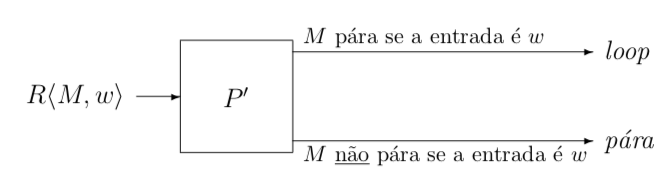
\includegraphics[scale=.4]{MTP1.png}
      \centering
    \end{figure}
    A partir de $P'$ podemos construir outra máquina, chamada $P^{''}$. Para
    construir $P^{''}$ a partir de $P'$ basta:
    \begin{enumerate}
      \item A partir da entrada $R\langle M \rangle$, gerar a palavra $R\langle
        M, R\langle M \rangle \rangle$, isto é, passaremos como entrada para a
        máquina $M$ o código correspondente a $M$, $R\langle M \rangle$.
      \item Agir como $P'$ sobre essa entrada.
    \end{enumerate}
    A seguir ilustramos a máquina $P^{''}$:
    \begin{figure}[H]
      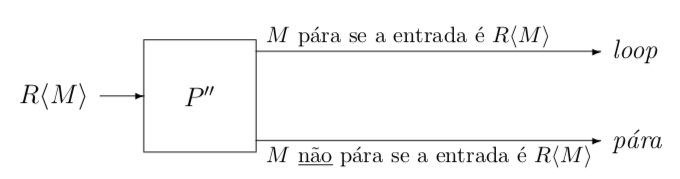
\includegraphics[scale=.4]{MTD.png}
      \centering
    \end{figure}
    De posse da MT $P^{''}$, podemos encontrar a contradição desejada. Considere
    o que acontece quando submetemos $R\langle P^{''} \rangle$ para a MT
    $P^{''}$:
    \begin{itemize}
       \item Se $P^{''}$ entra em loop com entrada $R\langle P^{''} \rangle$, é
         porquê $P^{''}$ para com entrada $R\langle P^{''} \rangle$;
       \item $P^{''}$ para com entrada $R\langle P^{''} \rangle$, é
         porquê $P^{''}$ entra em loop com entrada $R\langle P^{''} \rangle$;
    \end{itemize}
    Ou seja, $P^{''}$ para com entrada $R\langle  P^{''} \rangle$ se, e somente
    se,  $P^{''}$ não para com entrada $R\langle  P^{''} \rangle$, o que
    obviamente é uma contradição. Como podemos obter as MTs $P'$ e $P''$, a
    suposição inválida é a da existência de $P$. Portanto não existe MT capaz de
    resolver o problema da parada.
  \end{proof}

  \section{O Problema da Parada para Linguagens de Programação}
  
  \begin{Theorem}
    O problema da parada para linguagens de programação é indecidível.
  \end{Theorem}
  \begin{proof}
    Suponha que exista um procedimento \texttt{pare(x,w)} que dado um programa
    (expresso em texto) x e seus parâmetros de entrada (também expressos em
    texto) w, retorne verdadeiro se $x$ para com entrada w. Podemos escrever a
    seguinte função.
\begin{verbatim}
 procedimento D(x) {
    while (pare(x,x)) ;
 }
\end{verbatim}
    Seja $T$ o texto desse programa $D$. Então, se $D(T)$ para é  porquê
    \texttt{pare(T,T)}, retorna falso, o que significa que $D(T)$ não para;
    assim, se $D(T)$ para, $D(T)$ não! Por outro lado, se $D(T)$ não para é
    porque $P(T,T)$ é verdadeiro, o que significa que $D(T)$ pára. Assim,
    se $D(T)$ não pára, $D(T)$ para. Contradição! Dessa forma, conclui-se que o
    problema da parada para linguagens de programação é indecidível.
  \end{proof}

  \section{Consequência da Indecidibilidade do Problema da Parada}

  Considere a seguinte linguagem que representa as instâncias do problema da
  parada para MTs:

  \[
    L_P = \{R\langle M,w \rangle\,|\,M\textit{ para com entrada }w\}
  \]

  A seguir apresentamos algumas consequências da indecidibilidade de $L_P$.

  \begin{Theorem}
    A linguagem $L_P$ não é recursiva.
  \end{Theorem}
  \begin{proof}
    Consequência da indecidibilidade do problema da parada.
  \end{proof}

  \begin{Theorem}
    A linguagem $L_p$ é recursivamente enumerável.
  \end{Theorem}
  \begin{proof}
    Consequência da definição da MT universal, visto que $L_P$ é a linguagem
    aceita pela MT universal.
  \end{proof}

  \begin{Theorem}
    A linguagem $\overline{L_P}$ não é recursivamente enumerável.
  \end{Theorem}
  \begin{proof}
    Ora, se $\overline{L_P}$ fosse recursivamente enumerável, temos que $L_P$
    seria recursiva, o que é uma contradição.
  \end{proof}
  
  \section{Exercícios}

  \begin{enumerate}
     \item Prove que o problema de determinar se um programa P, em uma linguagem
       de programação qualquer, imprime a string ``Hello world!'' é indecidível.
     \item Mostre que se o problema da parada for decidível, então toda
       linguagem recursivamente enumerável seria recursiva.
  \end{enumerate}
\end{document}
